\section{Exploration on Behavior Data}
\subsection{Initial work}
\noindent
For behavior data, we wrote a function to merge three runs for each subject 
since we would like to look at the total observations within one subject.
Also we noticed that in the data set of each run, there existed observations
with "-1" in "respcat", which was meaningless and might be an error during 
the experiment so we took them out. For bold data, we also wrote a function 
to unzip all nii.gz files for further analysis.

\subsection{Behavior Data}
\noindent
We did some explanatory data analysis and regression analysis using behavior 
data. For explanatory data analysis, we generated some summary statistics, 
including correlation among variables and simple plots to better understand 
the behavior. And then we used regression analysis to mainly answer two 
scientific questions. The scientific questions that we have are:
\begin{itemize}
\item If gain/loss would be significant for individuals who choose to 
participate and how much time it would take for them to respond.
\item If gain/loss would be significant for whether individuals would like to 
participate in the gamble. 
\end {itemize}

\subsubsection {Linear regression}
To answer the first question, we built three linear regression models.
\begin{enumerate}
\item  Response Time $\sim$ gain + loss
\item  Response Time $\sim$ diff(gain-loss)
\item  Response Time $\sim$ ratio(gain/loss)
\end {enumerate}
\textbf{Result} \\
We use the result for one subject to explain our findings. In the first model, 
p value for the predictor loss is 0.002644 while p value for the predictor gain 
is 0.547262. Basically, we can conclude that people would actually care more 
about loss than gain. In the second model, p value for the predictor difference
is 0.413985.  It turns out that we can conclude that the difference between gain 
and loss wouldn't be a factor for how much time it would take for a individual 
to respond. In the third model, p value for the predictor ratio is extremely 
small, showing that ratio has a huge impact on individuals' response time.

\subsubsection {Logistic regression}
\noindent
To answer the second question, we fit logistic regression between Accept/Reject
Gamble and gain/loss. According to our analysis, the decision to whether take 
the gamble of most of subjects, in general, is more affected by loss amount 
rather than by gain amount.  For example, below is the analysis on the subject 
3. The regression line shows that it well follows the border between the two 
decisions: 1 (gamble) and 0 (not gamble). Right side of the line illustrates 
the decision to not gamble and it takes up more area relative to the opposite 
decision.
\begin{figure}[H]
    \centering
        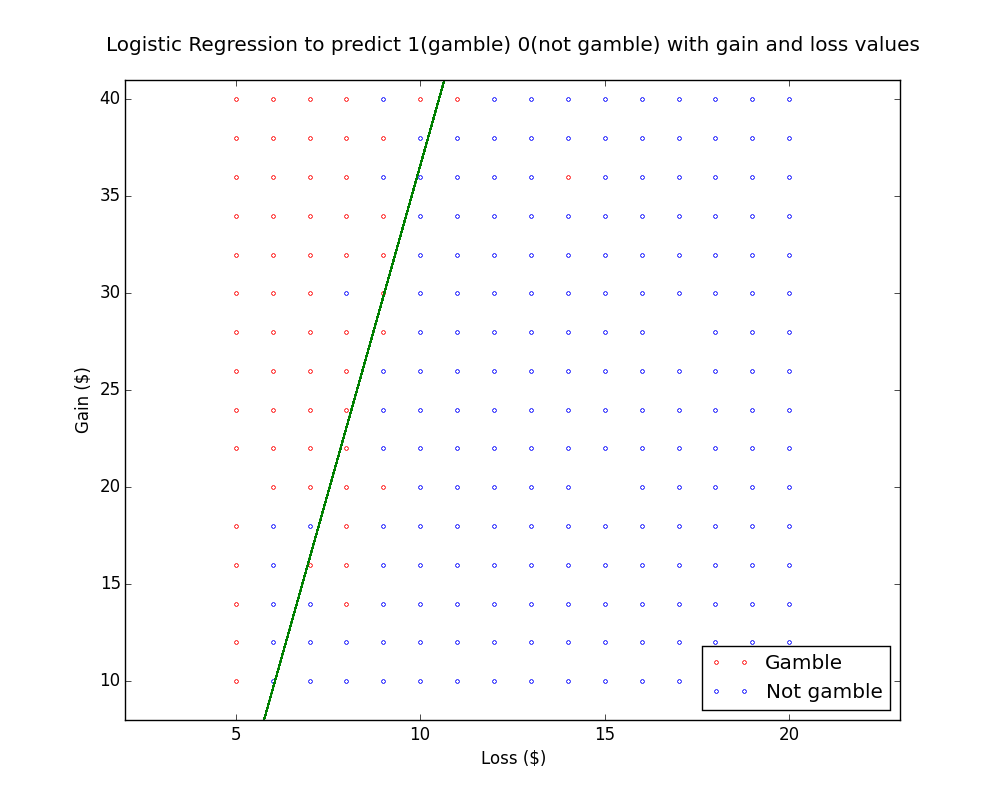
\includegraphics[scale=0.5]{log_regression.png}
    \caption{Logistic Regression for Subject 3}
\end{figure}



